\subsection{Autenticação por Radiofrequência}
\label{subsec:autenticacao-identificacao-radiofrequencia}

Os sistemas de identificação por radiofrequência ou~\acrfull{rfid} são uma
tecnologia
utilizada para recuperar informações automaticamente sobre produtos, pessoas ou
animais - ou seja, qualquer objeto em geral.
O objeto possui um pequeno circuito conhecido como \textit{tag}~\acrshort{
    rfid}, e os
dados registrados no meio podem ser recuperados automaticamente por um
dispositivo leitor.
Essa característica pode ser empregada em diversas aplicações industriais,
como rastreamento de itens ou sistemas de controle de acesso.
Além disso, os sistemas~\acrshort{rfid} não requerem contato, e nem precisam
estar
no campo de visão, utilizando a radiofrequência para transportar dados e energia
de forma eficiente\cite{feldhofer2004}.

\begin{figure}[h!]
    \caption[Estrutura de um sistema~\acrshort{rfid}]
    {Estrutura de um sistema~\acrshort{rfid}}
    \begin{tikzpicture}
    [
        action/.style={
            draw, thick, rectangle, rounded corners,
            text width=1.5cm, align=center,
        },
        action2/.style={
            draw, thick, double arrow,
            text width=1cm, align=center
        },
        snake/.style={
            -,
            decorate,
            decoration={
                snake,
                amplitude=1mm,
            }
        }
    ]
        \node[label={[below, yshift=-1.2cm,align=center]\textit{host}}](host){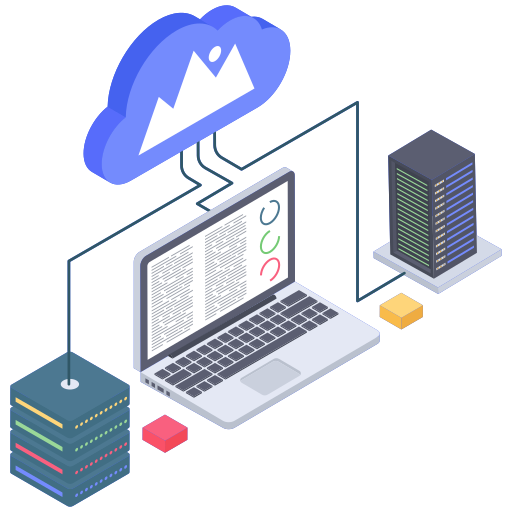
\includegraphics[width=0.1\textwidth]{graphics/host}};
        \node[action](reader)[right=0.8cm of host]{Leitor};
        \node[label={[above, align=center] Antena}](antenna)[right=0.1cm of
        reader]{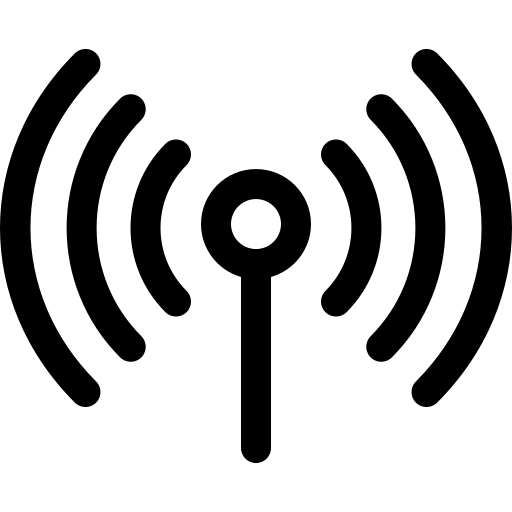
\includegraphics[width=0.05\textwidth]{graphics/antenna}};
        \node[action2](object)[right=0.3cm of antenna]{Dados \\ Energia \\
        Relógio};
        \node[action](tag)[right=1cm of object]{\textit{tag}}
        \node[label={[above, align=center] Antena}](antenna2)[left=0.1cm of
        tag]{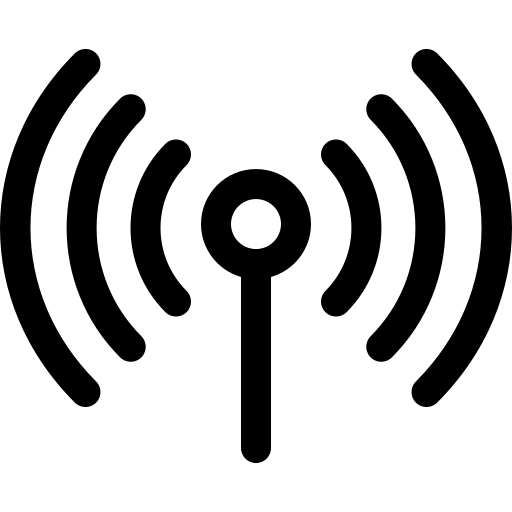
\includegraphics[width=0.05\textwidth]{graphics/antenna}};
        
        \draw (host) edge[snake] (reader);
    \end{tikzpicture}
    \label{fig:estrutura-sistema-rfid}
    \floatfoot{Adaptado de \cite{feldhofer2004}}
\end{figure}

Nos anos 50, os primeiros \textit{tags}~\acrshort{rfid} foram utilizados para
fins militares, embora fossem apenas para identificação.
Na época, sua função era limitada a transmitir sem fio um número serial
por ondas de rádio.
Nos últimos anos, os \textit{tags}~\acrshort{rfid} são um enorme sucesso na
indústria e seu uso se tornou generalizado.
As \textit{tags}~\acrshort{rfid} têm uma ampla gama de aplicações, incluindo
identificação de itens para dados de inventário, gerenciamento da cadeia de
suprimentos, telefones com capacidades~\acrshort{rfid} e autenticação de cartões
de plástico.
Acredita-se que as pessoas dependem da Internet para tudo e os \textit{tags}~\acrshort{rfid}
ajudarão nessa transição, dando capacidades de comunicação a produtos
cotidianos\cite{idrus2013}.

A segurança e o custo são duas desvantagens do~\acrshort{rfid}.
Embora o custo do~\acrshort{rfid} seja relativamente baixo em comparação com
outros sistemas de identificação, ainda é um pouco mais caro do que os sistemas
de código de barras convencionais.
As \textit{tags}~\acrshort{rfid} são vulneráveis a múltiplos ataques, representando
um risco de privacidade.
Portanto, muitos acadêmicos enfrentam o desafio de aumentar a segurança do~\acrshort{rfid},
enquanto mantêm o baixo custo das \textit{tags}~\acrshort{rfid}, determinando o
melhor método de autenticação\cite{jadhao2018}.